\documentclass[conference]{IEEEtran}
\usepackage{cite}
\usepackage{amsmath,amssymb}
\usepackage{graphicx}
\usepackage{booktabs}
\usepackage{array}
\usepackage{url}
\usepackage[hidelinks]{hyperref}

\begin{document}

\title{Fitur Klasik pada Tiga Kasus Pengolahan Citra Digital: Kematangan Sawit, Penyakit Daun Padi, dan Retak Jalan}

\author{\IEEEauthorblockN{Radistha Kriska Dahana Purusa}
\IEEEauthorblockA{NIM 561345\\
Pengolahan Citra Digital, Universitas Gadjah Mada\\
Email: radisthakriskadahanapurusa@mail.ugm.ac.id}}

\maketitle

\begin{abstract}
Laporan ini membandingkan tiga kasus pengolahan citra digital (PCD) berbasis
fitur klasik: kematangan tandan buah segar (TBS) sawit, penyakit daun padi, dan
retak jalan. Fitur warna (HSV, CIELab), tekstur (GLCM, LBP), bentuk, dan tepi
diklasifikasikan dengan SVM RBF dan Random Forest di CPU. Validasi memakai
$k$-lipat berstrata ($k=5$, tiga pengacakan), \emph{scaler} di dalam
\emph{pipeline}, dan pembagian per citra pada retak jalan. Macro-F1
terbaik adalah $0{,}858\pm0{,}062$ (sawit, tiga kelas, 150 citra),
$0{,}858\pm0{,}079$ (padi, tiga kelas, 120 citra), dan $0{,}868\pm0{,}022$
(retak jalan, \emph{patch} 64$\times$64 dari 118 citra). Fitur yang cocok berbeda per kasus: warna (sawit), warna, bentuk, dan
tekstur (padi), serta tepi dan morfologi garis (retak). Simpangan baku besar
pada dua kasus pertama, sehingga selisih kecil tidak bermakna.
\end{abstract}

\begin{IEEEkeywords}
pengolahan citra digital, ekstraksi fitur, SVM, Random Forest, pertanian, inspeksi jalan
\end{IEEEkeywords}

\section{Pendahuluan}
Pipeline PCD umumnya terdiri atas akuisisi, peningkatan mutu, segmentasi,
ekstraksi fitur, dan pengenalan~\cite{gonzalez2018}. Pada masalah terapan,
pemilihan fitur dan cara evaluasi sering lebih menentukan daripada
pengklasifikasinya. Laporan ini menguji hal itu pada tiga kasus dengan data
publik dan pengklasifikasi yang sama.

\section{Tiga Kasus, Data, dan Fitur yang Cocok}

\textbf{Kasus 1: kematangan TBS sawit.} Penilaian kematangan di pabrik masih
banyak dilakukan secara visual dan mempengaruhi rendemen minyak; sistem visi
warna untuk tugas ini sudah dikembangkan sejak lama~\cite{fadilah2012} dan
ditinjau oleh Lai \emph{et al.}~\cite{lai2023}. Data: \emph{Outdoor Tenera Oil
Palm Fruit}~\cite{omar2024}. Dari 1,1~GB data, dipakai subset seimbang 150 citra
(50 per kelas: \emph{unripe}, \emph{ripe}, \emph{overripe}), diambil acak
(\emph{seed} 0) dari gabungan folder latih dan uji; kelas \emph{damaged} dan
\emph{empty} dibuang karena terlalu sedikit. Fitur yang cocok adalah warna,
karena pematangan mengubah pigmen eksokarp dari gelap ke merah-jingga:
rata-rata, simpangan baku, dan \emph{skewness} kanal HSV (hue dipetakan ke
$\cos/\sin$) dan $L^*a^*b^*$ (21 fitur) pada piksel buah, ditambah tekstur GLCM
dan LBP (14 fitur). Lihat juga~\cite{rosbi2024}.

\textbf{Kasus 2: penyakit daun padi.} Data: UCI \emph{Rice Leaf Diseases}
(120 citra, 3 kelas @40: \emph{bacterial leaf blight}, \emph{brown spot},
\emph{leaf smut}). Penyakit dibedakan oleh warna, sebaran, dan bentuk bercak
sehingga fitur yang dipakai berupa momen warna daun dan lesi (21+21), 7
deskriptor bentuk lesi (luas relatif, jumlah, \emph{eccentricity},
\emph{solidity}, \emph{extent}, rasio sumbu), dan tekstur (14). Lesi diambil
dengan ambang kanal $a^*$ di dalam daun. Ekstraksi fitur untuk klasifikasi penyakit daun padi dibahas pada~\cite{azim2021}.

\textbf{Kasus 3: retak jalan.} Data: CrackForest~\cite{shi2016} (118 citra
$480\times320$ dengan anotasi piksel). Citra dipotong menjadi \emph{patch}
$64\times64$ tanpa tumpang tindih; \emph{patch} berlabel retak bila memuat
$\ge 30$ piksel retak, \emph{patch} dengan 1--29 piksel dibuang sebagai ambigu.
Hasilnya 4.034 \emph{patch} (1.235 retak, 2.799 non-retak). Retak adalah garis
gelap tipis sehingga fitur yang cocok adalah tepi dan morfologi garis: Canny dan
magnitudo Sobel, respons \emph{ridge} Sato, panjang \emph{skeleton} (9 fitur),
ditambah tekstur GLCM/LBP (16 fitur). Pra-pengolahan: median dan CLAHE. Rujukan deteksi retak:~\cite{zou2012,shi2016}.
Tekstur:~\cite{haralick1973,ojala2002}; warna:~\cite{woebbecke1995,gijsenij2011}.

\section{Metode Eksperimen}
Kode ada di \texttt{exp/} (CPU; scikit-image, scikit-learn, OpenCV). Citra sawit diubah ke $256\times256$, padi ke sisi
terpanjang 1024 piksel. Mask sawit memakai jarak Lab terhadap median tepi
citra, Otsu, morfologi, dan komponen terbesar. Dua pengklasifikasi dipakai:
SVM RBF ($C=10$, $\gamma=$ \texttt{scale}) dan Random Forest (200 pohon), keduanya
\texttt{class\_weight=balanced} dengan \texttt{StandardScaler} di dalam
\emph{pipeline} sehingga statistik hanya dihitung dari data latih tiap lipatan.
Validasi: \emph{stratified}
5-lipat untuk sawit dan padi; \emph{StratifiedGroupKFold} dengan grup $=$ citra
untuk retak jalan, dan keterpisahan citra latih/uji diperiksa dengan
\emph{assertion}. Semua dijalankan untuk tiga \emph{seed} (15 lipatan);
dilaporkan macro-F1 rata-rata $\pm$ simpangan baku antar lipatan.

\begin{figure*}[t]
\centering
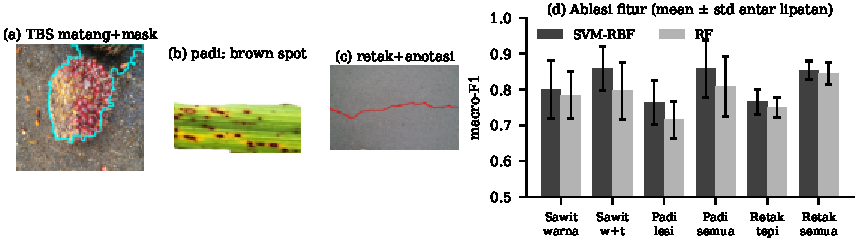
\includegraphics[width=0.96\textwidth]{results/fig_overview.pdf}
\caption{(a)--(c) Contoh citra tiap kasus: TBS dengan kontur mask, daun padi
\emph{brown spot}, dan retak jalan dengan anotasi (merah). (d) Macro-F1 pada
ablasi fitur; batang galat adalah simpangan baku antar lipatan.}
\label{fig:overview}
\end{figure*}

\section{Hasil}
\begin{table}[t]
\caption{Macro-F1 (rata-rata $\pm$ simpangan baku, 15 lipatan). Cetak tebal:
terbaik per kasus.}
\label{tab:res}
\centering
\footnotesize
\setlength{\tabcolsep}{3pt}
\begin{tabular}{@{}llcc@{}}
\toprule
\textbf{Kasus} & \textbf{Fitur} & \textbf{SVM RBF} & \textbf{RF} \\
\midrule
Sawit & Warna, tanpa mask & $0{,}804\pm0{,}063$ & $0{,}753\pm0{,}088$ \\
 & Warna, mask & $0{,}799\pm0{,}082$ & $0{,}784\pm0{,}066$ \\
 & Tekstur saja & $0{,}656\pm0{,}065$ & $0{,}672\pm0{,}072$ \\
 & Warna + tekstur & $\mathbf{0{,}858}\pm0{,}062$ & $0{,}796\pm0{,}080$ \\
\midrule
Padi & Warna daun utuh & $0{,}824\pm0{,}098$ & $0{,}780\pm0{,}107$ \\
 & Warna lesi & $0{,}764\pm0{,}062$ & $0{,}715\pm0{,}051$ \\
 & Bentuk lesi & $0{,}680\pm0{,}090$ & $0{,}694\pm0{,}103$ \\
 & Tekstur & $0{,}760\pm0{,}069$ & $0{,}630\pm0{,}096$ \\
 & Lesi + bentuk & $0{,}814\pm0{,}053$ & $0{,}762\pm0{,}091$ \\
 & Lesi + bentuk + tekstur & $\mathbf{0{,}858}\pm0{,}079$ & $0{,}810\pm0{,}084$ \\
\midrule
Retak & Tepi (Canny/Sobel) & $0{,}765\pm0{,}035$ & $0{,}751\pm0{,}028$ \\
 & Tepi + \emph{ridge} + morfologi & $\mathbf{0{,}868}\pm0{,}022$ & $0{,}840\pm0{,}026$ \\
 & Tekstur (GLCM + LBP) & $0{,}787\pm0{,}020$ & $0{,}778\pm0{,}027$ \\
 & Semua & $0{,}854\pm0{,}025$ & $0{,}844\pm0{,}031$ \\
\bottomrule
\end{tabular}
\end{table}

Pada sawit, warna saja ($0{,}80$) jauh lebih baik daripada tekstur saja
($0{,}66$), dan gabungan keduanya terbaik ($0{,}858$). Mask tidak memberi
perbaikan yang jelas pada SVM ($0{,}799$ vs.\ $0{,}804$). Galat terbanyak ada
antar kelas berdekatan (SVM, akumulasi 3 \emph{seed}: 21 \emph{ripe} diprediksi
\emph{unripe}, 17 \emph{overripe} diprediksi \emph{ripe}).
Pada padi, gabungan terbaik; bentuk lesi saja lemah ($0{,}68$). Pada retak jalan, fitur tepi/\emph{ridge}/morfologi ($0{,}868$) mengungguli
tepi sederhana ($0{,}765$) dan tekstur ($0{,}787$); menambah tekstur ke semua
fitur tidak memperbaiki hasil ($0{,}854$).

\section{Pembahasan}
\textbf{Kebocoran.} Pada retak jalan, \emph{patch} dari citra yang sama sangat
mirip. Pembagian acak per \emph{patch} memberi macro-F1 $0{,}867$ (SVM) dan
$0{,}849$ (RF) untuk semua fitur, lebih tinggi daripada $0{,}854$ dan $0{,}844$
dengan pembagian per citra: selisih kecil, tetapi searah dengan kebocoran.

\textbf{Batasan.} (i) Dataset kecil: dengan simpangan baku 0,06--0,10, selisih sekitar 0,05
(mis.\ SVM vs.\ RF) tidak dapat disimpulkan. (ii) Pada padi, warna daun utuh ($0{,}824$) mengungguli warna lesi
($0{,}764$); ini bisa mencerminkan kondisi akuisisi, dan citra dari daun yang sama
mungkin ada di lipatan latih dan uji karena tidak ada ID daun. (iii) Sawit tanpa ID kebun atau blok, sehingga validasi antar-kebun
tidak dapat diuji. (iv) Segmentasi lesi dan mask memakai ambang heuristik tanpa validasi
anotasi. (v) \emph{Patch} retak hanya 30\%, sehingga dipakai macro-F1. Hasil
tidak sebanding langsung dengan makalah rujukan.

\section{Kesimpulan}
Fitur klasik dengan SVM RBF atau Random Forest menghasilkan macro-F1 sekitar
0,86 pada ketiga kasus. Fitur yang cocok bergantung pada penyebab visual
kelasnya: warna untuk kematangan sawit, kombinasi warna lesi, bentuk, dan tekstur
untuk penyakit padi, serta tepi dan morfologi garis untuk retak jalan. Pada data sekecil ini perbedaan antar-pengklasifikasi tidak bermakna;
pemisahan per citra dan \emph{scaler} di dalam \emph{pipeline} menjadi syarat
evaluasi yang valid.

\begin{thebibliography}{99}
\scriptsize
\bibitem{gonzalez2018}
R.~C. Gonzalez and R.~E. Woods, \emph{Digital Image Processing}, 4th ed.
New York, NY, USA: Pearson, 2018.

\bibitem{fadilah2012}
N.~Fadilah, J.~Mohamad-Saleh, Z.~Abdul~Halim, H.~Ibrahim, and S.~S.~Syed~Ali,
``Intelligent color vision system for ripeness classification of oil palm
fresh fruit bunch,'' \emph{Sensors}, vol.~12, no.~10, pp.~14179--14195, 2012.

\bibitem{lai2023}
J.~W. Lai, H.~R. Ramli, L.~I. Ismail, and W.~Z. Wan~Hasan, ``Oil palm fresh
fruit bunch ripeness detection methods: A systematic review,''
\emph{Agriculture}, vol.~13, no.~1, p.~156, 2023.

\bibitem{omar2024}
Z.~Omar, A.~P.~P. Abdul~Majeed, M.~Rosbi, S.~A. Ghazalli, and H.~Selamat,
``Outdoor oil palm fruit ripeness dataset,'' \emph{Data in Brief}, vol.~55,
art.~110667, Aug. 2024.

\bibitem{rosbi2024}
M.~Rosbi, Z.~Omar, U.~Khairuddin, A.~P.~P.~A. Majeed, and S.~A.~R.~S.~A. Bakar,
``Machine learning for automated oil palm fruit grading: The role of fuzzy
C-means segmentation and textural features,'' \emph{Smart Agric. Technol.},
vol.~9, art.~100691, Dec. 2024.

\bibitem{azim2021}
M.~A. Azim, M.~K. Islam, M.~M. Rahman, and F.~Jahan, ``An effective feature
extraction method for rice leaf disease classification,'' \emph{TELKOMNIKA},
vol.~19, no.~2, p.~463, Apr. 2021.

\bibitem{shi2016}
Y.~Shi, L.~Cui, Z.~Qi, F.~Meng, and Z.~Chen, ``Automatic road crack detection
using random structured forests,'' \emph{IEEE Trans. Intell. Transp. Syst.},
vol.~17, no.~12, pp.~3434--3445, Dec. 2016.

\bibitem{zou2012}
Q.~Zou, Y.~Cao, Q.~Li, Q.~Mao, and S.~Wang, ``CrackTree: Automatic crack
detection from pavement images,'' \emph{Pattern Recognit. Lett.}, vol.~33,
no.~3, pp.~227--238, Feb. 2012.

\bibitem{haralick1973}
R.~M. Haralick, K.~Shanmugam, and I.~Dinstein, ``Textural features for image
classification,'' \emph{IEEE Trans. Syst., Man, Cybern.}, vol.~SMC-3, no.~6,
pp.~610--621, Nov. 1973.

\bibitem{ojala2002}
T.~Ojala, M.~Pietik\"ainen, and T.~M\"aenp\"a\"a, ``Multiresolution gray-scale
and rotation invariant texture classification with local binary patterns,''
\emph{IEEE Trans. Pattern Anal. Mach. Intell.}, vol.~24, no.~7, pp.~971--987,
Jul. 2002.

\bibitem{woebbecke1995}
D.~M. Woebbecke, G.~E. Meyer, K.~Von~Bargen, and D.~A. Mortensen, ``Color
indices for weed identification under various soil, residue, and lighting
conditions,'' \emph{Trans. ASAE}, vol.~38, no.~1, pp.~259--269, 1995.

\bibitem{gijsenij2011}
A.~Gijsenij, T.~Gevers, and J.~van~de~Weijer, ``Computational color constancy:
Survey and experiments,'' \emph{IEEE Trans. Image Process.}, vol.~20, no.~9,
pp.~2475--2489, Sep. 2011.

\end{thebibliography}
\end{document}
